% Welche Datenbank wurde verwendet und warum,...
\subsection{Anforderungen}
Es wird eine moderne Plattform entwickelt, auf der sich Nutzer ähnlich Social Media Profile anderer Nutzer anschauen und miteinander Chats führen. Nutzer sollen in Echtzeit miteinander schreiben können und nahezu keine Wartezeit in Kauf nehmen müssen, um sich andere Profile anzeigen zu lassen. Die Datenbank muss nahezu immer erreichbar sein, da Nutzer unsere Webseite sonst nicht nutzen können. 
Wenn Benutzer Änderungen an ihrem Profil vornehmen, kann eine geringe Wartezeit in Kauf genommen werden. Nutzer müssen bei Profilen nicht unbedingt die aktuelleste, gerade veränderte Profilbeschreibung sehen; es ist viel wichtiger, dass die Nutzer Nutzerprofile schnell sehen, all dass diese auf dem neuesten Stand sind. 
Webseiten wie unsere können "über Nacht" zum Erfolg werden, es reicht ein großer Influencer, welcher seinen Followern von der Webseite berichtet und auf einen Schlag erreichen wir Nutzerzahlen, bei denen unsere Rechenleistung auf Grenzen stößt. Die Datenbank unserer Wahl sollte sich vor allem schnell, ohne viel Programmieraufwand, skalieren lassen, um die Zeit, in denen unsere Plattform ausgelastet ist, möglichst gering zu halten. 
Statt dass unsere Nutzer ihr Verhalten auf unsere Webseite anpassen müssen, wollen wir die Webseite auf die Wünsche unserer Nutzer anpassen. Datenstrukturen sollen sich schnell und oft ändern können, um dies zu ermöglichen.

\subsection{Wahl der Datenbank}
In der näheren Auswahl der Datenbank standen die SQL-Datenbank PostgreSQL und MongoDB, eine NoSQL-Datenbank, zwei beliebte Datenbankmanagementsysteme mit unterschiedlichen Ansätzen. Wir werden uns im Folgenden die Gemeinsamkeiten und Unterschiede der Datenbanken anschauen und erklären, warum wir MongoDB als die für unser Projekt beste Lösung halten.

\subsubsection{PostgreSQL}
Michael Stonebreaker veröffentlichte 1974 in Berkeley unter BSD-Lizenz das RDBMS INGRES. Jahre später führte er das Projekt als Postgres (Post INGRES) weiter und fügte einen objektorientierten Ansatz hinzu. \cite{PG1} Im Laufe der Jahre wurde PostgreSQL fortlaufend weiterentwickelt und hat viele neue Funktionen dazuerhalten.
PostgreSQL beschreibt sich selbst als \enquote{das fortschrittlichste, quelloffene, relationale Datenbankmanagementsystem und habe sich in über 30 Jahren aktiver Entwicklung einen guten Ruf für Zuverlässlichkeit, Funktionsrobusheit und Leistung verdient}. \cite{PG2} PostgreSQL soll auch in Zukunft unter einer quelloffenen Lizenz stehen, welche die kommerzielle Nutzung erlaubt. \cite{PG3}
PostgreSQL wurde exemplarisch als Option eines SQL-Systems verwendet, da der Funktionsumfang vergleichbar mit anderen beliebten SQL-Systemen ist. \cite{PG4}

\subsubsection{MongoDB}
Die 2007 neu gegründete Firma 10Gen, mittlerweile bekannt als MongoDB Inc., benötigte eine Datenbank, welche den Anforderungen ihrer quelloffenen Plattform-as-a-Service Cloud-Architektur gerecht werden würde. Das Team suchte nach einer Datenbank, die elastisch, skalierbar, einfach zu verwalten und für Entwickler und Anwender einfach zu benutzen ist. Unzufrieden mit den zu der Zeit auf dem Markt verfügbaren Datenbanksystemen wurde MongoDB, eine dokumentbasierte Datenbank entwickelt. Als das Team das Potenzial der Datenbank realisierte, wurde die Idee der Cloud-Plattform eingestellt und die Entwicklung von MongoDB gefördert.\cite{MG1}
Laut eigenen Aussagen ist \enquote{MongoDB [] eine universelle, dokumentbasierte, verteilte Datenbank für die moderne Anwendungsentwicklung und die Cloud, die in puncto Produktivität höchsten Ansprüchen gerecht wird}. \cite{MG2} 


\subsubsection{MongoDB und PostgreSQL im Vergleich}

\begin{center}
    \begin{tabularx}{\linewidth}{ |X|X|X| } 
     \hline
     Kriterien & PostgreSQL & MongoDB  \\ 
     \hline
     Datenbanktyp & SQL, Objektrelational & NoSQL, Dokumentbasiert \\
     Ranking nach DB-Engines \cite{DB1} & 577,50 Punkte, viertbeliebteste Datenbank, viertbeliebteste relationale Datenbank & 496,50 Punkte, fünftbeliebteste Datenbank, beliebteste nicht-relationale Datenbank \cite{DB2} \\
     Architektur & Monolithisch & Dezentralisiert \\
     Erscheinungsjahr & 1989 & 2009 \\
     Datenschema & Ja & Selbstbeschreibende Dokumente\\
     Referenzierung & Referenzierung per ID, erlaubt Foreign Keys & Referenzierung per ID oder eingebettetes Sub-Dokument \\
     Datenstruktur & Tabellen bestehen aus Zeilen und Spalten & Kollektionen bestehen aus Dokumenten. Dokumente haben Felder. Dokumente der gleichen Kollektion müssen nicht die selben Felder besitzen. \\
     Typisierung & Erlaubt verschiedene Datentypen und nutzerdefinierte Datentypen\cite{PG5} & Erlaubt verschiedene Datentypen nach BSON Spezifikation \cite{MG3}; ähnelt stark JSON \\
     Horizontale Skalierung & Repliken nach Master-Slave-System \cite{PG6} & Sharding und Replica Sets als Teil der Infrastruktur \cite{MG4} \cite{MG5} \\
     Konsistenzmodell & ACID, optional eventuelle Konsistenz \cite{MG6} \cite{MG7} & ACID \\
     \hline
    \end{tabularx}
    \cite{DB3} \cite{DB4}
\end{center}

\subsubsection{ACID}
 MongoDB ist seit Erschaffung auf Dokumentebene ACID-Konform und ab den Versionen 4.0 (Juni 2018 \cite{MG8}) auf einem einzelnen Replik-Set bzw. ab Version 4.2 (August 2019 \cite{MG8}) zwischen mehreren Replik-Sets bei multi-Dokument-Transaktionen ACID-Konform. \cite{MG6} Dies erlaubt "Alles-oder-Nichts"-Transaktionen, bei denen es kritisch ist, dass entweder alle Teile oder kein Teil der Transaktion ausgeführt wird und löst damit Probleme, die historisch nur mit SQL-Datenbanken lösbar waren.

\subsubsection{Referenzierung und Denormalisierung}
PostgreSQL erlaubt, andere Tabellen mit Foreign Keys (FK) gemäß SQL-Standard zu referenzieren. Der Wert eines FK muss korrekt sein, sollte der angegebene FK in der referenzierten Tabelle nicht existieren, wird ein Fehler geworfen. Auch ist es möglich, entsprechende Regeln zu definieren, was passieren soll, wenn der referenzierte Datensatz beispielsweise gelöscht wird.
MongoDB ermöglicht auch, andere Dokumente per ID zu referenzieren, bietet jedoch keine direkte Option, zu definieren, was beim Löschen des referenzieren Datensatzes passieren soll. Es ist weiterhin möglich, Trigger beim Löschen des referenzierten Datensatzes feuern zu lassen, dies hat im Vergleich zum Foreign Key Constraint allerdings eine höhere Komplexität. Stattdessen setzt MongoDB darauf, alle relevanten Informationen soweit möglich in einem Dokument einzubetten.
%TODO Schaubilder erstellen 1-1 1-Many Many-Many

Eingebettete Dokumente erlauben schnelleren Lesezugriff, da sich alle relevanten Informationen in einem Dokument befinden und - anders als in SQL - nicht über mehrere Tabellen mit im Laufe des Produktlebenszyklus immer komplexeren JOIN-Anweisungen zusammengefasst werden müssen. Dies vereinfacht das Schreiben von Abfragen und erhöht die Geschwindigkeit von Leseabfragen. Als Nachteil wird dabei in Kauf genommen, dass Daten über verschiedene Dokumente dupliziert werden und Schreibzugriffe dadurch langsamer werden - schließlich müssen Daten in verschiedenen Dokumenten erstellt oder aktualisiert werden. 
Jedes Mal, wenn das Profil eines Nutzers in der Kontaktsuche angezeigt werden soll oder wenn die Freundesliste oder ein Chat geöffnet wird, muss das Profil dieses Nutzers abgefragt werden. Das kann teilweise für hunderte Anfragen pro Profil am Tag sorgen und belastet entsprechend unsere Datenbank. Den Projektanforderungen nach ist außerdem wichtig, dass Nutzer schnell Profile angezeigt bekommen. Schreibanfragen, bei denen ein neues Profil erstellt wird oder ein Nutzer sein eigenes Profil aktualisiert, werden weitaus seltener vorkommen als Leseanfragen. Auch sind wir der Meinung, dass Nutzer eine längere Wartezeit bei Profilaktualisierungen eher hinnehmen, als bei Lesezugriffen zu warten.
Entsprechend sind wir der Meinung, dass für unser Projekt die Vorteile eingebetteter Dokumente dessen Nachteile überwiegen.

\subsubsection{Skalierbarkeit}
Sowohl PostgreSQL als auch MongoDB lassen sich vertikal skalieren - mit mehr Ressourcen läuft die Datenbank schneller. Bei horizontaler Skalierung verfolgen die beiden Datenbanken verschiedene Ansätze.
\paragraph{PostgreSQL} nutzt ein Master-Slave-System bzw. Primary-Standby-System mit Lastverteilung.\cite{PG6} Die Standby-Knoten sind Kopien des Primärknotens und können Lesezugriffe verarbeiten. Schreibzugriffe werden nur vom Primärknoten angenommen. Sollte der Primärknoten versagen, bietet PostgreSQL keine automatische Lösung dieses Problems, ohne Drittsoftware muss manuell ein neuer Primärknoten gewählt werden. Es gibt nur einen Primärknoten, für Multi-Master-Systeme wird Drittsoftware benötigt. Selbst mit synchronen Repliken dauert es einen Moment, bis die Standby-Knoten die Aktualisierungen der Datenbank übernommen haben, dies kann dazu führen, dass Abfragen mit veralteten Datensätzen beantwortet werden.\cite{PG8} Consistency nach CAP-Theorem ist für PostgreSQLs Master-Slave-Systeme somit nicht mehr einhundertprozentig gegeben.
Durch Sharding lässt sich die Datenbank in einzelne Knoten aufteilen, die jeweils nur einen Teil der Daten beinhalten. Dies erlaubt es, die Last und benötigte Speicherkapazität pro Knoten weiter zu verringern. Es ist möglich, mehrere Shards vom gleichen Knoten verwalten zu lassen; dies erleichtert die Skalierung, da die Anzahl der Shards flexibel an die technischen Ressourcen des verwaltenden Knoten angepasst werden kann.
\paragraph{MongoDB}
benutzt Replik-Sets, welche ähnlich wie das vorgestellte Master-Slave-System von PostgreSQL funktionieren. Der Primärknoten ist der einzige Knoten mit Schreibzugriff und repliziert die Änderungen auf die Sekundärknoten. Alleridngs hat MongoDB ein automatisches System, welches einen Ausfall des Primärknotens abfängt. Alle Knoten teilen den anderen Knoten ihren \enquote{Herzschlag} mit, in dem sie sich gegenseitig anpingen. Sollte der Herzschlag des Primärknotens ausfallen, wählen die Sekundärknoten unter ihnen einen neuen Primärknoten aus, welcher dann die Aufgaben des früheren Primärknotens übernimmt. Es ist möglich, Knoten mit mehr Rechenleistung eine höhere Priorität zuzuweisen, um die Wahrscheinlichkeit zu erhöhen, dass dieser Knoten der nächste Primärknoten wird. Auch ist es möglich, zu verhindern, dass spezielle Knoten Primärknoten werden, dies ist ratsam für Knoten, die schlechtere Hardware besitzen oder eine höhere Latenz aufweisen, weil sie beispielsweise in einer entfernten Region stehen. Den Knoten können zudem verschiedene Rollen zugewiesen werden, versteckte Knoten können für Datenbankauswertungen verwendet werden, während verzögerte Knoten einen historischen Schnappschuss der Datenbank speichern und Aktualisierungen der Datenbank mit einer Verzögerung ausführen und somit als Backup dienen können. \cite{MG10}\cite{MG11}\cite{MG12}\cite{MG13} MongoDB erlaubt zudem Systeme mit mehreren Primärknoten, in den meisten Fällen sind Optionen wie Sharding jedoch besser geeignet. \cite{MG14}
Shards wiederum können als eigene Replica-Sets eingesetzt werden. Dies erlaubt es, für verschiedene Regionen eigene Shards der Datenbank einzurichten, welche dann wiederum in einem eigenen Replica-Set gesteuert werden.

\begin{figure}[ht]
	\centering
    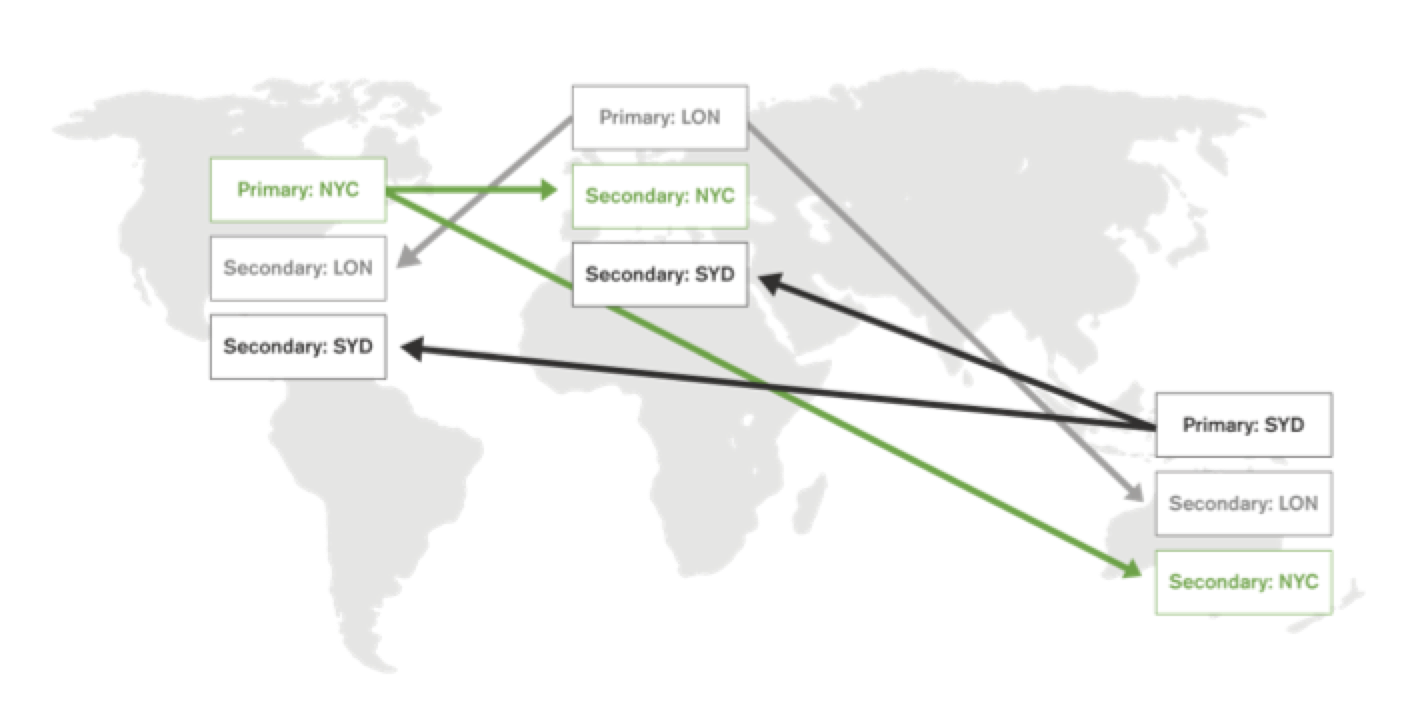
\includegraphics[width=\textwidth]{sources/MongoDB_sharded.png}\cite{MG14}
	\caption{Aktiv-Aktiv-Architektur mit Datenbank-Sharding}
	\label{fig1}
\end{figure}

Jedes Jahr fallen größere Mengen an Daten an. Durch diese Entwicklung ist die Möglichkeit, horizontal skalieren zu können, immer wichtiger geworden. Zur Anfangszeit von PostgreSQL hat es für die meisten Projekte gereicht, vertikal zu skalieren, erst über die Jahre wurden Techniken zur horizontalen Skalierung entwickelt. Für Techniken wie der automatischen Wahl eines neuen Primärknotens oder Multi-Master-Systemen benötigt es Drittsoftware. In MongoDB ist horizontale Skalierung seit jeher wichtige Priorität und ist als solches stark in die Datenbankinfrastruktur eingebettet. Wir sind der Meinung, dass die von MongoDB verwendeten Lösungen zur horizontalen Skalierung ausgereifter sind und gleichzeitig weniger fachliches Wissen benötigen und damit entsprechend schneller und einfacher durchführbar sind.

\subsubsection{Flexibilität}
Wir haben die Erfahrung gemacht, dass vor allem in der Anfangsphase von Projekten Datenbankstrukturen oft angepasst und verworfen werden. MongoDB nutzt Kollektionen, dessen Dokumente nicht die exakt gleiche Strutur aufweisen müssen, anders als dies bei einer ORDBMS-Tabelle wie bei PostgreSQL der Fall ist. Diese Flexibilität ermöglicht es, die Datenbank schnell auf sich wechselnde Projektziele anpassen zu können und erhöht somit die Geschwindigkeit, mit der an agilen Projekten gearbeitet werden kann. Dabei ist darauf zu achten, dass die Datenbankänderungen nicht zu mehr Problemen führen, als sie lösen. Sollte dieses Risiko beachtet werden, eignet sich MongoDB für unser Projekt in diesem Punkt besser als PostgreSQL.

\subsubsection{Das CAP-Theorem}
%TODO gut schreiben
Brewers CAP-Theorem sagt aus, dass es in verteilten Systemen wie Datenbanken nicht möglich ist, gleichzeitig Consistency (Konsistenz), Availability (Verfügbarkeit) und Partition Tolerance (Partitionstoleranz) zu gewährleisten. Man muss sich für zwei entscheiden. %cite paper
% https://awoc.wolski.fi/dlib/big-data/GiLy02-CAP.pdf AXIOM
% https://groups.csail.mit.edu/tds/papers/Gilbert/Brewer2.pdf
% https://www.researchgate.net/publication/220476881_CAP_Twelve_years_later_How_the_Rules_have_Changed (download CAP-computer)
%TODO weiter recherchieren https://de.wikipedia.org/wiki/CAP-Theorem
Dies ist eine starke Simplifizierung, die den heutigen Datenbanken in der Form nicht gerecht wird und zwölf Jahre später von Brewer angepasst wurde. 
Viele aktuelle Datenbanken erlauben es, in unterschiedlichen Konfigurationen verschiedene Ziele zu erreichen und auch wenn weiterhin nur zwei der drei Ziele vollständig erfüllt werden können, ist das CAP-Theorem flexibler als ursprünglich angenommen

Wir haben am Fallbeispiel von PostgreSQL zeigen können, dass im Multiknoten-System ein Teil der Konsistenz aufgegeben werden kann, um kürzere Antwortzeiten und Partitionstoleranz (Standby-Knoten dürfen ausfallen) zu gewährleisten. Die Einführung eines Multi-Master-Systems würde eine Erhöhung der Partitionstoleranz (beliebige Knoten dürfen ausfallen) zu Kosten von Konsistenz (gleichzeitige Schreibzugriffe auf verschiedene Knoten) erwirken und somit das System Richtung AP-Datenbank verschieben. Synchrone Replizierung auf Standby-Knoten erhöht die Konsistenz, erhöht aber gleichzeitig die benötigte Zeit einer Operation und verringert somit die Verfügbarkeit, schiebt also somit den Fokus Richtung CP-Datenbank. Diese Funktionen sind in anderen Datenbanken in ähnlicherweise zu finden und erlauben aktuellen Datenbanken, fein auf die Anforderungen des Benutzers angepasst zu werden.

\subsubsection{Erfahrung}
Das Entwicklerteam hat in der Vergangenheit bereits Erfahrung in MongoDB sammeln können und ist gut mit der Datenbank zurecht gekommen. Die Entwickler wissen, wie die Datenbank funktioniert und auf was zu achten ist. Dies verringert das Risiko und spart Zeit, da die Technologie bereits bekannt ist.

\subsubsection{Dateiformat}
MongoDB speichert Daten im \glqq binary JSON\grqq -Format. JSON, die \glqq JavaScript Object Notation \grqq, ist \enquote{ein schlankes Datenaustauschformat, welches für Menschen einfach zu lesen und für Maschinen einfach zu parsen [] ist} \cite{JSON1}. JSON als semistrukturiertes Dateiformat eignet sich gut für Schnittstellendaten. Zudem wird im gewählten MERN-Techstack ausschließlich JavaScript verwendet - das JavaScript native Dateiformat JSON ist daher ohne Umwandlungen direkt verwendbar und der Umgang für unsere Entwickler bereits bekannt. Dies verringert die Gefahr möglicher Komplikationen und spart Lern- und Programmieraufwand.

\subsubsection{Beliebtheit}
Eine beliebte Datenbank zu wählen hat einige Vorteile. Beliebte Datenbanken werden meist aktiv weiterentwickelt, haben oft mehr Tools von Drittanbietern welche die Arbeit erleichern und haben meist eine aktive Programmierergemeinschaft, welche bei kleineren Problemen schnell aushelfen kann. Bei der Expandierung des Projekts gibt es zudem eine größere Auswahl an qualifiziertem Fachpersonal.
Nach dem Ranking von DB-Engines schneiden PostgreSQL und MongoDB ähnlich ab. PostgreSQL ist mit 577,50 Punkten die viertbeliebteste ORDBMS und insgesamt die viertbeliebteste Datenbank. MongoDB ist mit 496,50 Punkten die beliebteste Dokumentdatenbank und damit insgesamt die fünftbeliebteste Datenbank. Platz Eins bis Vier werden von ORDBMS-Datenbanken ein. \cite{DB4}
In der Entwicklerumfrage 2021 von StackOverflow kommt man auf ähnliche Ergebnisse. Von den 49.537 Befragten gaben 36,1\% an, PostgreSQL zu nutzen, während 26,4\% MongoDB nutzen. PostgreSQL landet damit auf Platz 2, MongoDB auf Platz 4. \cite{DB5}
Beide Datenbanken erfreuen sich großer Beliebtheit und werden allen Anschein nach noch etliche Jahre verwendet werden. Im NoSQL-Markt ist MongoDB am beliebtesten, während es im SQL-Markt weitere andere beliebte Datenbanken gibt. In diesem Aspekt hat keine Datenbank Vorteile gegenüber der Anderen.

\subsubsection{Fazit}
Wir haben nach einer Datenbank gesucht, welche bei Leseanfragen schnell antwortet, schnelle Änderungen der Datenstrukturen zulässt, eine hohe Erreichbarkeit aufweist und sich schnell und einfach skalieren lässt. Dafür nehmen wir langsamere Schreibanfragen und Inkonsistenz bei Leseanfragen in Kauf. Wir konnten zeigen, dass sowohl PostgreSQL als auch MongoDB ausgereifte Lösungen sind, sich MongoDB als Gesamtpaket für unsere speziellen Anforderungen besser eignet.
%Begründen

\subsection{Schemata}
Folgende Kollektionen wurden verwendet, um die Daten optimal zu verwalten.

\subsubsection{Nutzer}
\begin{center}
    \begin{tabularx}{\textwidth}{ |X|X|X| } 
     %\hline
     %Feld & Beschreibung & Beispiel \\ 
     %\hline
     % _id & Standardmäßige MongoId & \\
     % Benutzername & einzigartiger, öffentlicher Name & MaxMustermann \\ 
     % normalisierter Name & Name in Kleinbuchstaben. Wird verwendet, um die Einzigartigkeit von Namen zu gewährleisten & maxmustermann \\ 
     % Email & private eMail des Nutzers & mustermann@email.de \\
     % Rolle & Gibt an, ob der Nutzer autorisiert ist - Moderatoren und Administratorkonten haben mehr Rechte. Automatisch generiert & Nutzer \\ 
     % Geburtsdatum & privates Geburtsdatum des Nutzers & 01.01.2000 \\ 
     % Alter & Alter des Nutzers. Wird automatisch mit Geburtsdatum berechnet & 21 \\ 
     % Sprachen & Array von Sprachen, die der Nutzer sprechen kann & [de, en] \\
     % Geschlecht & gesellschaftliches Geschlecht des Nutzers. & Männlich \\ 
     % Spielposition & Bis zu 2 Lieblingspositionen des Spielers in League of Legends & [Mid, Jungle] \\ 
     % Freitext & kurzer Text, in dem der Nutzer sich beschreiben kann. & Ich bin ein toller Nutzer! \\
     % Avatar & URI [GLOSSAR!] vom Avatarbild des Nutzers & https://<s3-name>.s3.eu-central-1.amazonaws.com/avatars/<UUID>.jpg \\ 
     % Freunde & Array von allen Freunden des Nutzers. Beinhaltet die NutzerID und die ChatID & [[_id1, NutzerID1, ChatID1], [_id2, NutzerID2, ChatID2]]\\ 
     % Geblockt & Array von NutzerIDs der Nutzer, die geblockt wurden & [NutzerID3, NutzerID4] \\ 
     %\hline
    \end{tabularx}
\end{center}

Wenn ein Nutzer einen Account erstellt, gibt dieser dessen eMail, den gewünschten Benutzernamen und das gewünschte Passwort an. Durch Indexe wird die Einzigartigkeit von eMail und Benutzername geprüft, das Passwort wird aus Sicherheitsgründen in einer separaten Kollektion gespeichert. Nach der Kontoerstellung kann der Nutzer das Geburtsdatum, die gesprochenen Sprachen, das Geschlecht, die Spielposition und einen Freitext angeben und ein Bild hochladen, welches als Avatarbild dient. Felder wie der normalisierte Name, das Alter und die Rolle werden automatisch generiert. Im Laufe der Nutzung unserer Plattform wird der Nutzer andere Spieler als Freunde hinzufügen - diese werden in einer Freundesliste gespeichert. Auch steht es dem Nutzer frei, Andere zu blockieren - in diesem Fall wird die NutzerID des Blockierten auf die Blockliste hinzugefügt.
Privatsphäre und damit die Sicherheit der eigenen Daten ist uns wichtig. Wir wollen daher die Anzahl an Daten, die ein Nutzer von sich preisgeben müssen, so gering wie möglich halten. Die Email-Adresse, das Geburtsdatum und Freundes- und Blockliste sind für andere Nutzer nicht einsehbar, bis auf den Benutzernamen muss eine Person keine Daten öffentlich angeben.

\subsubsection{Sprache}
Damit Nutzer ihre Sprache wählen können, bieten wir die Wahl zwischen 187 Sprachen nach ISO 639-1 Norm an.\cite{ISO639-1} 

\begin{center}
    \begin{tabular}{ |c|c|c| }
        \hline
        Feld & Beschreibung & Beispiel \\
        \hline
        id & Alpha-2 Code der Sprache & en, de, fr \\
        name & Englische Schreibweise der Sprache & English, German, French \\
        nativer Name & native Schreibweise der Sprache & English, Deutsch, français \\
        \hline
    \end{tabular}
\end{center}
Normale Objekt-IDs von MongoDB enthalten einen Zeitstempel und einen inkrementellen Zähler.\cite{MG15} Diese Daten halten wir bei Sprachen, also öffentlichen Stammdaten, die sich über einen langen Zeitraum nicht verändern werden, nicht sinnvoll. Stattdessen haben wir den Alpha-2-Code der Sprache als ID gewählt, der auf die Sprache schließen lässt. Nutzerdokumente referenzieren die Sprache per ID, dies erlaubt es uns, direkt im Nutzerdokument anhand der Sprach-ID zu erkennen, welche Sprachen der Nutzer spricht.
Sprachen können sowohl anhand der englischen Schreibweise als auch der nativen Schreibweise gefunden werden. Dies erleichtert Nutzern auch nicht-englischsprachigen Nutzern, ihre Sprache auswählen zu können.

\subsubsection{Passwort}
\begin{center}
    \begin{tabular}{ |c|c| }
        \hline
        Feld & Beschreibung  \\
        \hline
        id & Standardmäßige MongoId \\
        password & Bcrypt Hash bestehend aus Versionsnummer, Komplexität, Salt und Hash \\
        NutzerID & MongoId des zugehörigen Nutzers \\
        \hline
    \end{tabular}
    \cite{DB3} \cite{DB4}
\end{center}

Das Passwort wird nicht im Nutzerdokument gespeichert. Würde das Passwort im Nutzerdokument gespeichert werden, könnte es schon durch kleine Programmierfehler dazu kommen, dass normale Nutzer das gehashte Passwort anderer Nutzer ermitteln könnten. Um dieses Sicherheitsproblem direkt zu eliminieren, wird daher für jedes Passwort ein eigenes, vom Nutzerdokument isoliertes Dokument verwendet.
Das Passwort wird durch bcrypt, einem Blowfish-basiertem Hashalgorithmus, auf der Datenbank als Hash mit Salt gespeichert. Die Komplexität des Hashes ist durch uns wählbar. Bei der Wahl der Komplexität ist die Sicherheit gegen Rechengeschwindigkeit abzuwägen; eine höhere Komplexität erhöht die benötigte Zeit pro Versuch eines Angreifers, das Passwort zu knacken, erhöht gleichzeitig aber auch die Zeit, die unser Server benötigt, um ein neues Passwort zu generieren oder den Anmeldeversuch eines ehrlichen Nutzers zu bestätigen. Eine zu hohe Komplexität kann daher unseren Server stark verlangsamen und macht Angriffszenarien per (D)DOS gefährlicher, da gezielte Anmeldeversuche viel Last auf dem Server erzeugen.
Um die Wahrscheinlichkeit von Glückstreffern bei Angriffen zu verringern, verlangen wir außerdem, dass das Passwort mindestens aus 8 Zeichen, darunter 1 Großbuchstabe, 1 Kleinbuchstabe und 1 Ziffer erstellt wird. Für mehr Varianz in den Passwörtern sind zudem einige Sonderzeichen erlaubt.
Durch gewählte Restriktionen besteht eine 1:1-Relation zwischen Passwörtern und Nutzerkonten.

\subsubsection{Like}
\begin{center}
    \begin{tabular}{ |c|c| }
        \hline
        Feld & Beschreibung  \\
        \hline
        id & Standardmäßige MongoId \\
        Sender & NutzerID der Person, die den Like/Dislike versendet. \\
        Empfänger &  NutzerID der Person, die den Like/Dislike empfängt. \\
        Status & Gibt an, ob es sich um einen Like oder Dislike handelt. \\
        \hline
    \end{tabular}
    \cite{DB3} \cite{DB4}
\end{center}

Der Name "Like" für diese Datenstruktur ist irreführend, da in der Kollektion sowohl Likes als auch Dislikes (angegeben durch den Status) gespeichert werden.
Immer wenn ein Nutzer bei der Kontaktsuche angibt, ob er mit einer Person Kontakt aufnehmen oder diesen vermeiden will, wird ein Dokument angelegt. Wenn der Nutzer in Kontakt treten will, wird zusätzlich geprüft, ob bereits ein Datensatz existiert, bei dem Sender und Empfänger vertauscht sind - ob sich also die Nutzer gegenseitig einen Like gegeben haben. Sollte das der Fall sein, werden beide Datensätze gelöscht und die Nutzer zur Freundesliste des jeweils anderen hinzugefügt. in dem Fall können die Nutzer miteinander kommunizieren.

\subsubsection{Chat}
\begin{center}
    \begin{tabular}{ |c|c| }
        \hline
        Feld & Beschreibung  \\
        \hline
        id & Standardmäßige MongoId \\
        Teilnehmer & Array von NutzerIDs, die dem Chat beiwohnen. Aktuell maximal 2. \\
        Nachrichten & Array von Nachrichten, die die Nutzer untereinander ausgetauscht haben. \\
        \hline
    \end{tabular}
    \cite{DB3} \cite{DB4}
\end{center}
Wenn zwei Nutzer sich befreunden, wird ein Chat zwischen diesen erstellt. Wenn ein Nutzer die Freundschaft beendet, verlässt dieser Nutzer gleichzeitig den Chat. Mit der gewählten Struktur sind auch Gruppenchats ohne Änderung der Datenbank möglich, für die Projektanforderungen steht diese Funktion jedoch nicht im Fokus.
Um Ressourcen zu sparen, wird bei der Standard-Datenbankabfrage nur die neueste Nachricht geladen. Diese Abfrage dient für Vorschaubilder des Chats in der Kontaktliste. Außerdem ist es möglich, durch Seitennummerierung (Pagination) je Abfrage 20 Nachrichten zu erfragen. Diese Methoden verringern die Serverlast, meist reicht es Nutzern, die letzten 20 Nachrichten eines Chats zu lesen.
Nachrichten sind eingebettete Dokumente eines Chats. Sie weisen folgende Datenstruktur auf:

\paragraph{Nachricht}
\begin{center}
    \begin{tabular}{ |c|c| }
        \hline
        Feld & Beschreibung  \\
        \hline
        id & Standardmäßige MongoId \\
        Inhalt & Text der Nachricht \\
        Autor & NutzerID des Verfassers der Nachricht \\
        \hline
    \end{tabular}
    \cite{DB3} \cite{DB4}
\end{center}

\subsection{Database-as-a-Service}
Um eine Datenband selbst zu betreiben fehlen uns Kapazitäten und eine Infrastruktur. Wir sind daher auf eine Database-as-a-Service-Lösung (DBaaS) angewiesen. 
MongoDB Inc. bietet mit MongoDB Atlas eine Database-as-a-Service Lösung an, die Flexibel auf die Größe und Auslastung des Projektes angepasst werden kann. Dazu gibt es verschiedene Datenbankstufen, die mit höheren Kosten mehr Rechenleistung und weitere Funktionen erhält. Zwischen den Stufen kann flexibel gewechselt werden, um den aktuellen Anforderungen gerecht zu werden. Kostenpflichtige Stufen bieten die Möglichkeit an, Backups einzurichten, ab Stufe M10 stehen Tools zur Verfügung, die Metriken in Echtzeit anzeigen, automatisch archivieren, Empfehlungen zur Leistungsoptimierung erstellen und langsame Datenbankabfragen zur Diagnose anzeigen. In der Entwicklungsphase haben wir uns für die kostenlose Stufe entschieden, da die Funktionen und Leistung dafür ausreichen. Sollte das Produkt auf den Markt gehen, werden wir die kostengünstigste Stufe wählen, um die Option von Backups zu erhalten. Wenn das Projekt erfolgreich ist und wir viele Nutzer anziehen, wird flexibel, abhängig von benötigter Leistung, eine höhere Stufe gewählt.
Sowohl die Produktions-, als auch die Entwicklungsumgebung werden als eigene Datenbanken von MongoDB Atlas gehosted. Dies verringert das Risiko von Code, der auf der lokalen Maschine funktioniert, aber auf der Produktionsumgebung Fehler wirft. Durch die Nutzung gleicher Werkzeuge und gleicher Technologie wird die Werkzeuglücke verringert und dementsprechend die Dev-Prod-Vergleichbarkeit erhöht. \cite{12FA1}

Diese lassen sich schnell einrichten, fallen selten aus und werden automatisch mit Updates versorgt. Es stehen Reportingtools zur Verfügung, die das Auswerten der Datenbank erleichern. DBaaS spart viel administrativen Aufwand und verringert damit die Kosten.

\section{Avatarbilder}
Statt Bilddateien für Avatare direkt auf der Datenbank zu speichern, speichern wir nur URIs zu den Bildern auf unserer Datenbank. Die Bilder selbst werden auf AWS S3 gehosted, einem Speichersystem, welches für BLOB-Dateien optimiert ist. Dies nimmt der Datenbank Last ab und erhöht die Anfragegeschwindigkeit bei Lese- und Schreibzugriffen des Avatarbildes. Der S3-Speicher wurde so eingerichtet, dass das Backend Zugriffsrechte zum erstellen und löschen von Dateien hat. Es wurde dabei mit Minimalprinzip vorgegangen, damit ein möglicher Angriff auf unser System die geringsten Schäden im Erfolgsfall verursacht, hat unser Backend nur die nötigsten Zugriffsberechtigungen auf S3. Die Datenbank wird mithilfe von GraphQL angesprochen, für S3 hat sich diese Lösung jedoch nicht angeboten. Für das Hochladen von Profilbildern wurde eine weitere Route im Backend erstellt, bei der mit den npm-Packeten Multer und Multer-S3 kontrolliert wird, ob es sich bei der vom Nutzer hochgeladenen Datei um eine Bilddatei handelt und ob diese eine bestimmte Bildgröße nicht übersteigt.

\section{Fazit}
Mit den gewählten Kollektionen und der Wahl von speziellen Hosts sind wir in der Lage, Nutzern eine Datenbank zu geben, die eine hohe Erreichbarkeit aufweist, leicht zu skalieren ist, personenbezogene Daten geheim hält und ein Maß an Datensicherheit bietet, welches der größe des Projektes entspricht. Durch eingebettete Dokumente, Denormalisierung und Seitennummerierung wurden Optimierungen durchgeführt, die als Ziel haben, möglichst schnell Antworten auf Leseanfragen zu bieten.


